\chapter{Romberg quadrature}

\section{The algorithm}

Let \(f:[a,b] \rightarrow \R\) be a function and \(I\coloneqq \int_a^bf(x)dx\). The {\it trapezoidal rule} is a method for approaching \(I\) which works as follows: Let \(a = t_0 < t_1 < \cdots < t_n = b\) be a subdivision of \([a,b]\). On each of the intervals \([t_{i-1},t_i]\) we approximate \(\int_{t_{i-1}}^{t_i}f(x)dx\) by the area of a trapezoid with verticies \((t_{i-1},0),\,(t_{i-1}, f(t_{i-1})),\,(t_i,f(t_i)),\, (t_i,0)\) i.e. by \(\frac{1}{2}(t_i - t_{i-1})(f(t_{i-1}) + f(t_i))\). Hence we approximate \(I\) by 

\[
I = \sum_{i=1}^n \int_{t_{i-1}}^{t_i}f(x)dx \approx \sum_{i=1}^n\frac{1}{2}(t_i - t_{i-1})(f(t_{i-1}) + f(t_i)).
\]
If \(t_i - t_{i-1} = \frac{1}{n}(b-a)\eqqcolon h\) for each \(i\) then the above estimate becomes
\begin{equation}\label{trapezoidal}
I \approx h \left(\frac{1}{2}(f(a) + f(b)) + \sum_{i=1}^{n-1}f(a + ih)\right)
\end{equation}
We define \(T_f(h)\) as the right hand side in (\ref{trapezoidal}).\\

Let \(F:[0, n]\rightarrow \R\) be a \(2k+1\) times continuously differentiable function, \(n\) a positive integer. Then by Euler's summation formula (see formula 298 in \cite{kn}) we have
\begin{equation}
\sum_{i=0}^nF(i) = \int_0^nF(x)dx + \frac{1}{2}(F(0) + F(n)) + \sum_{i=1}^k\frac{B_{2i}}{(2i)!}(F^{(2i-1)}(n) - F^{(2i-1)}(0)) + R_k
\end{equation}
where \(R_k = \int_0^nP_{2k+1}(x)F^{(2k+1)}(x)dx\), \(B_m\) are the {\it Bernoulli numbers} and \(P_m\) the {\it Bernoulli polynomials.} If let \(F(x)\coloneqq f(a + xh)\) then we get the following asymptotic expansion for the trapezoidal rule:

\begin{theorem}
Let \(f:[a,b] \rightarrow \R\) be \(2k+1\) times continuously differentiable and \(h \coloneqq (b-a)/n\). Then 
\begin{equation}
T_f(h) = I + \sum_{i=1}^k\frac{B_{2i}}{(2i)!}(f^{(2i-1)}(b) - f^{(2i-1)}(a))h^{2i} + h^{2k+1}R_k(h)
\end{equation}
where
\begin{equation}
R_k(h) = \int_a^bP_{k+1}\left(n\frac{x-a}{b-a}\right)f^{(2k+1)}(x)dx. 
\end{equation}
\end{theorem}

The following code is a trivial implementation of the trapezoidal rule. The {\it TrapezoidalRule} class in an implementation of the abstract class {\it Scheme} which represents a numerical scheme or method, which has asymptotic expansion in \(h^p\). The Scheme class has a method named {\it apply} which takes in a problem to which the scheme is applied to. The argument \(m\) in the apply-method is the number of subintervals that should be used.

\begin{minted}[tabsize=2, fontsize=\footnotesize]{python}
class TrapezoidalRule(Scheme):
    def __init__(self):
        super(TrapezoidalRule, self).__init__(2)

    def apply(self, inte, m):
        (a,b) = inte.interval
        h = (b - a) / m
        I = 0.5 * (inte.f(a) + inte.f(b))
        for i in range(1, m):
            I += inte.f(a + i * h)

        return I * h
\end{minted}

Assume that we have computed the value of \(T_f(h)\) for \(h = h_1,\ldots,h_k\) and we want extrapolate to zero, i.e. we want to compute the value at zero of the interpolation polynomial in \(h^2\) for \((h_i^2,T_f(h_i)\), \(i=1,\ldots,k\). Denote by \(T_{ij}\) the value at zero of the polynomial in \(h^2\) which goes through \((h_{i-j+1}^2, T(h_{i-j+1}),\ldots,(h_i^2,T(h_i))\). The Neville scheme gives us the following algorithm for computing \(T_{ij}\), \(1\leq j\leq i\leq k\), recursively:

\begin{enumerate}
    \item \(T_{i1} \coloneqq T_f(h_i)\) for \(i = 1,\ldots,k\).
    \item \(T_{ij} \coloneqq T_{i,j-1} + \frac{T_{i,j-1} - T_{i-1,j-1}}{\left(\frac{h_{i-j+1}}{h_i}\right)^2 - 1}\) for \(2\leq j\leq i\).
\end{enumerate}

\section{Numerical experiments}

In this section we are going to apply Romberg quadrature to various functions and also try different sequences. We will analyze how different sequences perform in the sense that we want to measure how many function evaluations we need to attain a prescribed precision.\\

We will try various functions and the following sequences:
\begin{itemize}
    \item The harmonic sequence: \(a_n = n\), \(n\geq 0\).
    \item The Romberg sequence: \(a_n = 2^{n-1}\), \(n\geq 1\).
    \item The Bulirsch sequence: \(a_1 = 1\), \(a_2 = 2\), \(a_3 = 3\) and \(a_{n+2} = 2\cdot a_n\) for \(n\geq 2\). Its first elements are 
    \[
    1,\, 2,\, 3,\, 4,\, 6,\, 8,\, 12,\, 16,\, 24,\, 32,\ldots
    \]
\end{itemize}
Suppose that we are approximating the integral \(I\coloneqq \int_a^b f(x)dx\) using Romberg quadrature. We will use the stepsizes \(h_k\coloneqq (b-a)/a_k\) for the extrapolation. Let \(T_{ij}\), \(i\geq 0\) and \(j\leq i\) be the extrapolation table we get and \(\varepsilon_k \coloneqq |T_{kk}-I|\) be the error on the diagnoals. Let \(N_k\) be the number of function evaluations needed to compute \(T_{kk}\). We will use \(N_k\) as the measurement of computational effort as mentioned in section 1.3 and we will try to fit the exponential convergence model introduced there. We will also plot the logarithm of the error against the number of extrapolation steps. Note that \(N_k = \sum_{i=1}^k(a_i + 1)\) where \((a_i)\) is our sequence, so in case of the Harmonic sequence, we have \(N_n = n(n+3)/2 \approx n^2/2\) for \(n\) large. Hence if \(\varepsilon_n \sim A\exp(-cN_n^q)\) then 
\[
\varepsilon_n \sim A\exp(-c/2^qn^{2q})
\]
for \(n\) large. Thus if the error converges exponentially with the number of function evaluations, it will also converge exponentially with the number of extrapolation steps, and the exponent in the latter fitting will be twice the parameter from the former.\\

If our sequence is the Romberg sequence then \(N_k = \sum_{i=1}^n (2^{i-1} + 1) = 2^k + k - 1 \approx 2^k\) for \(k\) large, so if \(\varepsilon_k\sim A \exp(-cN_k^q)\) then 
\[
\varepsilon_k \sim A\exp(-c 2^{kq}) 
\]
for \(k\) large, which is not exponential convergence. On the other hand, if the we have exponential convergence in the number of extrapolation steps, i.e.
\[
\varepsilon_k \sim A \exp(-c k^q)
\]
then since \(k \approx \ln N_k / \ln 2\) we get 
\[
\ln \varepsilon_k \sim \ln A - c (\ln N_k / \ln 2)^q = \ln A - \frac{c}{(\ln 2)^q} (\ln N_k)^q
\]
so if we consider the ln-ln plot of the error against the number of function evaluations, then the points should fall on the graph of a function of the form \(t\mapsto b - c t^q\). The exponent should be the same as in the fitting for the logarithm of the error against the number of extrapolation steps.\\

For the model fitting we will thus plot the logarithm of the error agains the number of function evaluations, the number of extrapolation steps and the logarithm of the number of extrapolation steps. We will also consider the plot of the base \(10\) logarithm of the error against the number of function evaluations.\\

In order to validate the fitting, we will do "cross validation" in the following way: We will estimate the parameters in the models where we only consider every other point, every third point and then when we only consider a consecutive sequence of half of the points, though never fewer than \(10\).\\ 

We conduct the experiments in Python 3 and use the high precision arithmetic library mpmath for all the computations. The precision will be set to \(500\) significant digits so will not have to worry about numerical instabilities.\\

Now we will consider the results of the experiments.

\subsection{Cosine squared}
The first function we are going to try is
\[
f: [0, \pi]\rightarrow \R, \quad f(x) \coloneqq \cos^2(x)
\]
which is entire.

%cos^2(x)
\begin{figure}[H]
\centering
\begin{minipage}{0.45\textwidth}
\centering
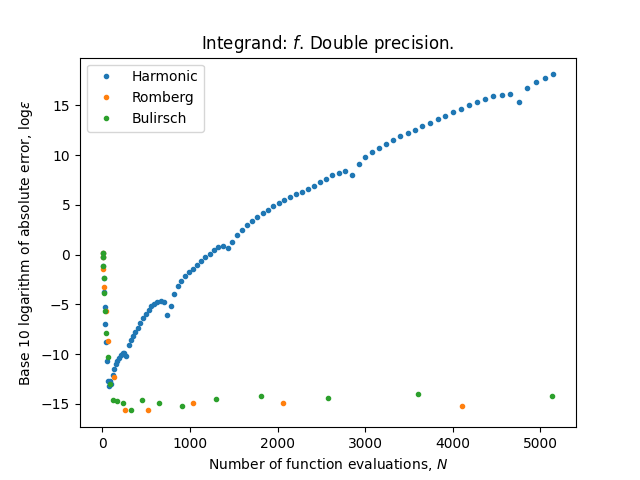
\includegraphics[scale=0.45]{romberg_plots/cos_squared.png}
\end{minipage}
\begin{minipage}{0.45\textwidth}
\centering
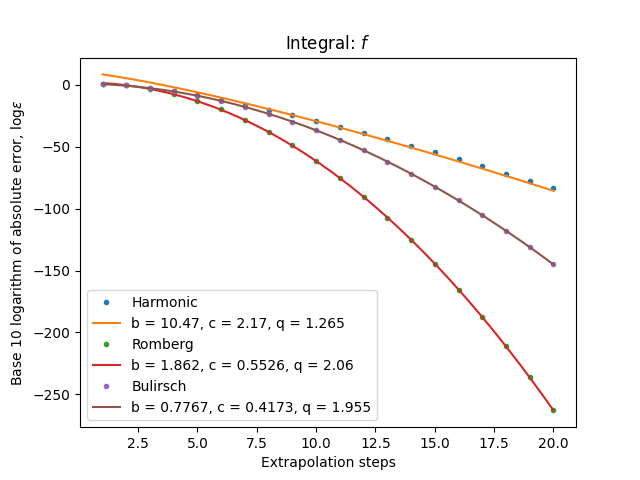
\includegraphics[scale=0.45]{romberg_plots/cos_squared_hp_steps.png}
\end{minipage}
\end{figure}

\begin{figure}[H]
\centering
\begin{minipage}{0.45\textwidth}
\centering
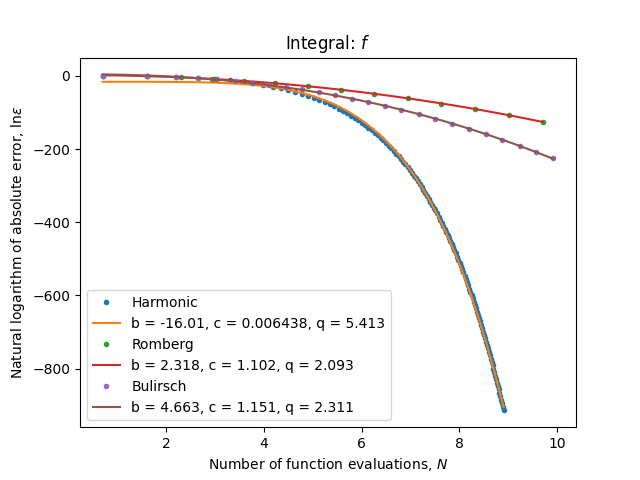
\includegraphics[scale=0.45]{romberg_plots/cos_squared_hp_log_log_pow_fit_trend.png}
\end{minipage}
\begin{minipage}{0.45\textwidth}
\centering
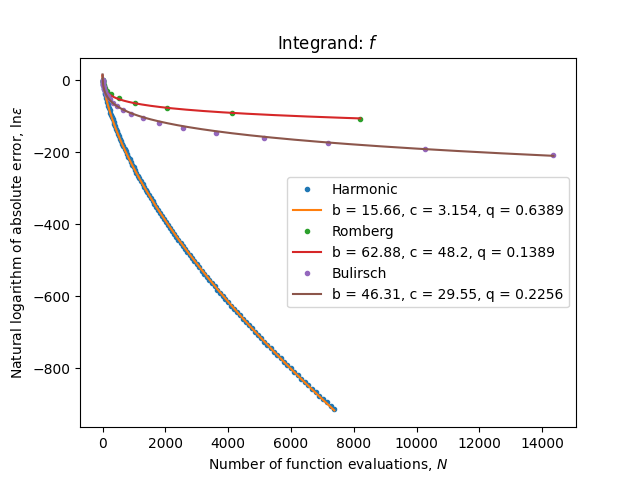
\includegraphics[scale=0.45]{romberg_plots/cos_squared_hp_trend.png}
\end{minipage}
\end{figure}

\begin{table}[H]
    \centering
    \begin{tabular}{c|c||c|c|c}
Sequence & Plot & \(A\)-variance & \(c\)-variance & \(q\)-variance\\\hline
Harmonic & lin-ln evals-error & \(15.892\) & \(0.052543\) & \(0.0037803\) \\
Romberg & lin-ln evals-error & \(3.9999\) & \(0.10449\) & \(0.029386\) \\
Bulirsch & lin-ln evals-error & \(14.911\) & \(0.43183\) & \(0.20258\) \\
Harmonic & lin-ln steps-error & \(14.477\) & \(0.03992\) & \(0.0021086\) \\
Romberg & lin-ln steps-error & \(0.066039\) & \(0.0010865\) & \(3.8422e-05\) \\
Bulirsch & lin-ln steps-error & \(0.18524\) & \(0.0019423\) & \(5.5812e-05\) \\
Harmonic & ln-ln evals-error & . & . & . \\
Romberg & ln-ln evals-error & \(0.031489\) & \(0.00052793\) & \(2.887e-05\) \\
Bulirsch & ln-ln evals-error & \(2.9654\) & \(0.088636\) & \(0.0071409\) \\
    \end{tabular}
    \label{tab:my_label}
\end{table}

We see that the harmonic sequence performes best, then Bulirsch and then Romberg. In standard double precision arithmetic, we get down to machine level precision using Romberg or Bulirsch, but we are like \(2\) digits from there, using the harmonic sequence.\\

For the Romberg and Bulirsch sequence, we can not say that the error converges exponentially with the number of function evaluations since the parameters we get in the cross validation vary a lot. In the case of the harmonic sequence, we seem to have exponential convergence in the number of function evaluations, though that must be verified better, since the \(b\) and \(c\) parameters vary quite much.\\

For all sequences the error seems to converge exponentially with the number of extrapolation steps, but again we there is a lot of variance in the \(b\) parameter.\\

As we expect, since the error seems to converge exponentially with the number of extrapolation steps, \(\ln\)-\(\ln\) plot for the Romberg and Bulirsch sequence seem to fit quit well on the graph of a function of the form \(t \mapsto b - c t^q\). On the other hand, that is not the case for the harmonic sequnce, as we expect.

\subsection{Function with poles}

Now we will consider the following function:
\[
g_a: [-1, 1] \rightarrow \R, \quad g_a(x) \coloneqq \frac{1}{a^2 + x^2},\, a > 0
\]
\begin{figure}[H]
\centering
\begin{minipage}{0.45\textwidth}
\centering
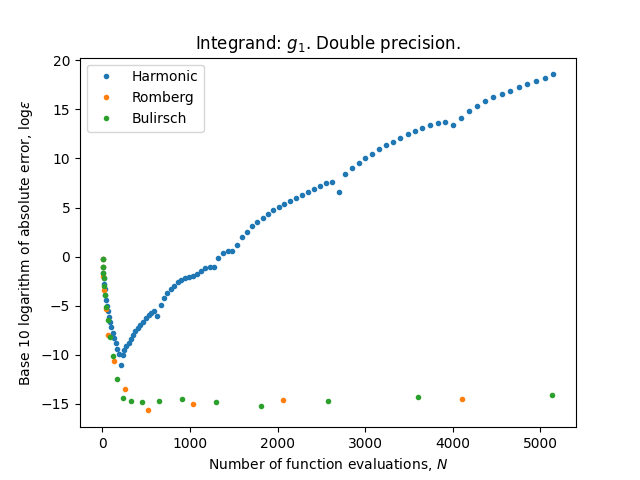
\includegraphics[scale=0.45]{romberg_plots/g_one.png}
\end{minipage}
\begin{minipage}{0.45\textwidth}
\centering
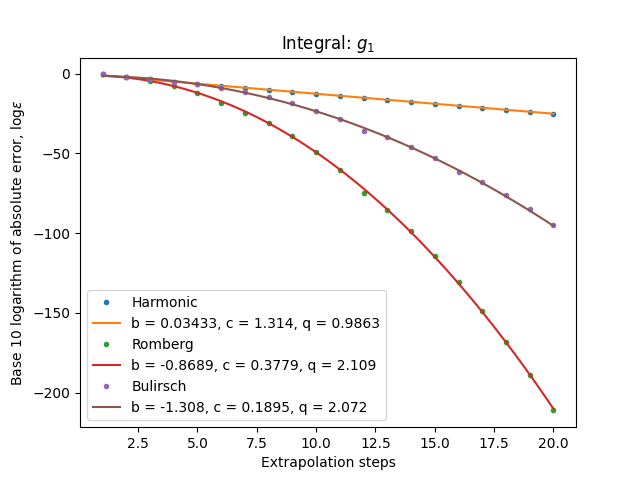
\includegraphics[scale=0.45]{romberg_plots/g_one_hp_steps.png}
\end{minipage}
\end{figure}

\begin{figure}[H]
\centering
\begin{minipage}{0.45\textwidth}
\centering
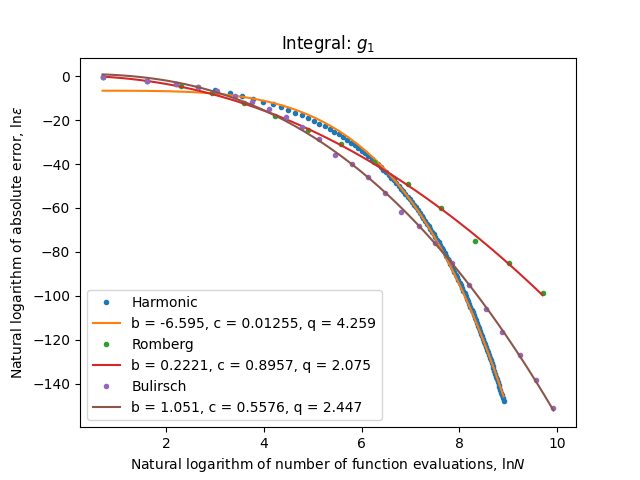
\includegraphics[scale=0.45]{romberg_plots/g_one_hp_log_log_pow_fit_trend.png}
\end{minipage}
\begin{minipage}{0.45\textwidth}
\centering
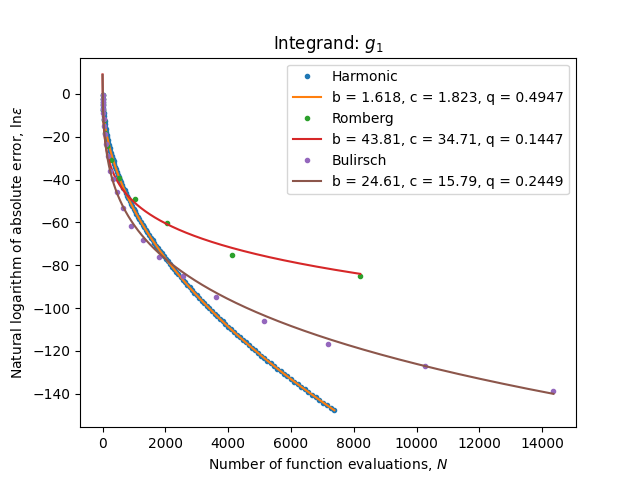
\includegraphics[scale=0.45]{romberg_plots/g_one_hp_trend.png}
\end{minipage}
\end{figure}

\begin{table}[H]
    \centering
    \begin{tabular}{c|c||c|c|c}
Sequence & Plot & \(A\)-variance & \(c\)-variance & \(q\)-variance\\\hline
Harmonic & lin-ln evals-error & \(0.091387\) & \(0.00065694\) & \(3.963e-05\) \\
Romberg & lin-ln evals-error & \(4\) & \(0.33642\) & \(0.085159\) \\
Bulirsch & lin-ln evals-error & \(nan\) & \(3.2071\) & \(0.58712\) \\
Harmonic & lin-ln steps-error & \(0.17361\) & \(0.001823\) & \(0.00010357\) \\
Romberg & lin-ln steps-error & \(1.8814\) & \(0.52416\) & \(0.035469\) \\
Bulirsch & lin-ln steps-error & \(15\) & \(1.7795\) & \(0.099758\) \\
Harmonic & ln-ln evals-error & . & . & . \\
Romberg & ln-ln evals-error & \(1.4183\) & \(0.45669\) & \(0.038901\) \\
Bulirsch & ln-ln evals-error & \(15\) & \(1.7737\) & \(0.14009\) \\
    \end{tabular}
    \label{tab:my_label}
\end{table}

We see that the harmonic sequence performes best, then Bulirsch and then Romberg. In standard double precision arithmetic, we get down to machine level precision using Romberg or Bulirsch, but we are like \(5\) digits from there, using the harmonic sequence.\\

For the Romberg and Bulirsch sequence, we can not say that the error converges exponentially with the number of function evaluations since the parameters we get in the cross validation vary a lot, especially since the exponent \(q\) varies a lot. In the case of the harmonic sequence, the model seems to fit very well, since we have very little variance in the parameters.\\

For all sequences the error seems to converge exponentially with the number of extrapolation steps, but again we there is quit a lot of variance in the \(b\) parameter. Note that the exponent from the fitting for the Harmonic sequence is twice the parameter we got when considering the number of function evaluations agains the error, as expected.\\

The model fits quite well to the \(\ln\)-\(\ln\) plot in the case of the Romberg sequence. It clearly does not fit for the Harmonic sequnce but fits moderately well for the Bulirsch sequence.

\begin{figure}[H]
\centering
\begin{minipage}{0.45\textwidth}
\centering
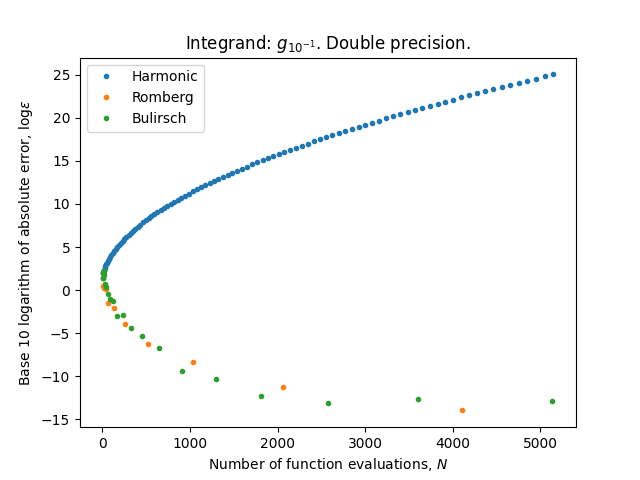
\includegraphics[scale=0.45]{romberg_plots/g_tenth.png}
\end{minipage}
\begin{minipage}{0.45\textwidth}
\centering
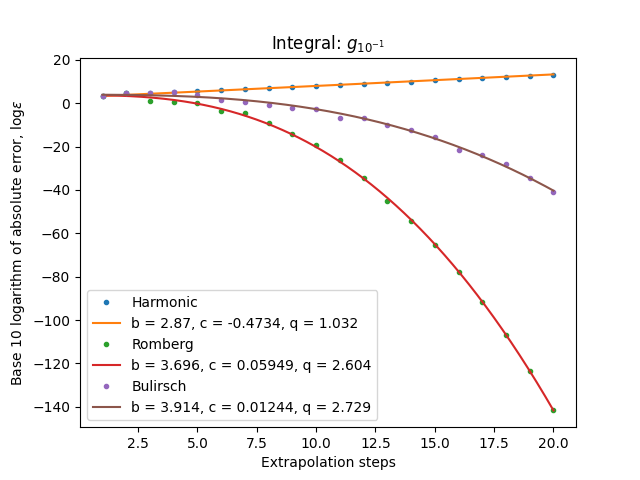
\includegraphics[scale=0.45]{romberg_plots/g_tenth_hp_steps.png}
\end{minipage}
\end{figure}

\begin{figure}[H]
\centering
\begin{minipage}{0.45\textwidth}
\centering
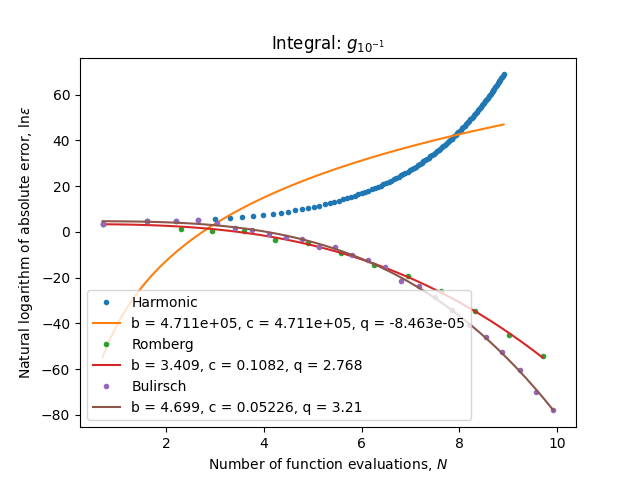
\includegraphics[scale=0.45]{romberg_plots/g_tenth_hp_log_log_pow_fit_trend.png}
\end{minipage}
\begin{minipage}{0.45\textwidth}
\centering
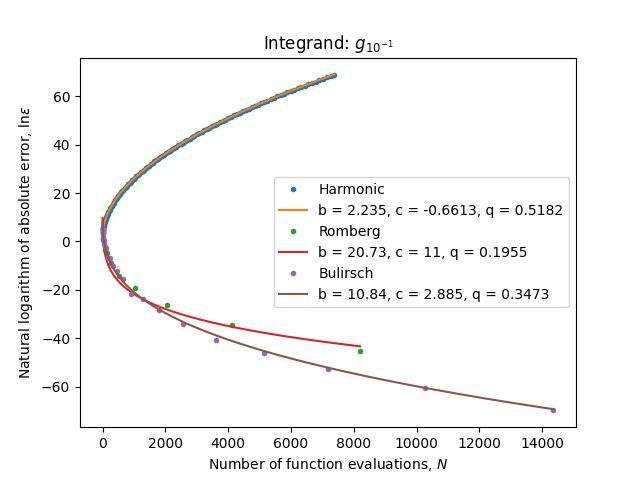
\includegraphics[scale=0.45]{romberg_plots/g_tenth_hp_trend.png}
\end{minipage}
\end{figure}

\begin{table}[H]
    \centering
    \begin{tabular}{c|c||c|c|c}
Sequence & Plot & \(A\)-variance & \(c\)-variance & \(q\)-variance\\\hline
Harmonic & lin-ln evals-error & \(0.66369\) & \(0.019182\) & \(0.0031665\) \\
Romberg & lin-ln evals-error & \(3.9854\) & \(0.30308\) & \(0.073011\) \\
Bulirsch & lin-ln evals-error & \(nan\) & \(14.616\) & \(0.74405\) \\
Harmonic & lin-ln steps-error & \(0.29415\) & \(0.014971\) & \(0.0018903\) \\
Romberg & lin-ln steps-error & \(1.5386\) & \(0.49618\) & \(0.012829\) \\
Bulirsch & lin-ln steps-error & \(nan\) & \(14.991\) & \(0.29893\) \\
Harmonic & ln-ln evals-error & . & . & . \\
Romberg & ln-ln evals-error & \(1.5752\) & \(0.4164\) & \(0.014402\) \\
Bulirsch & ln-ln evals-error & \(nan\) & \(14.981\) & \(0.33583\) \\
    \end{tabular}
    \label{tab:my_label}
\end{table}

Here we get divergence for the harmonic sequence, but convergence for the other sequences, fastest for Bulirsch. In standard double precision arithmetic, we get down to machine level precision using Romberg or Bulirsch.\\

For the models, in case of convergence, they do not fit very well in any case. The best fitting is when we consider the logarithm of the error against the number of extrapolation steps and the logarithm of number of function evaluations, for the Romberg sequence. There is though quite a lot of variance in the \(b\) and \(c\) parameters.

\begin{figure}[H]
\centering
\begin{minipage}{0.45\textwidth}
\centering
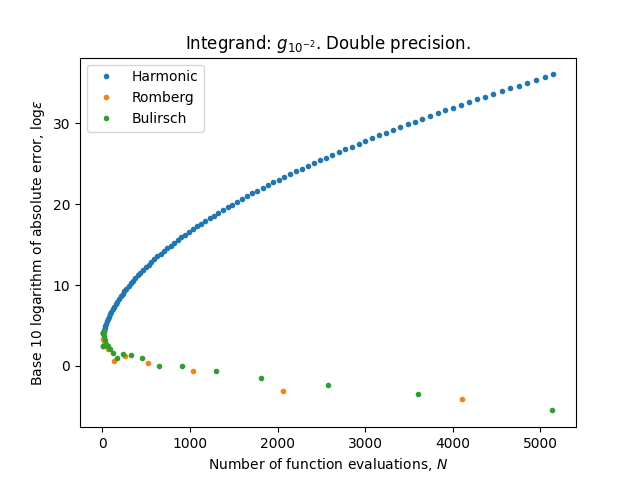
\includegraphics[scale=0.45]{romberg_plots/g_hundredth.png}
\end{minipage}
\begin{minipage}{0.45\textwidth}
\centering
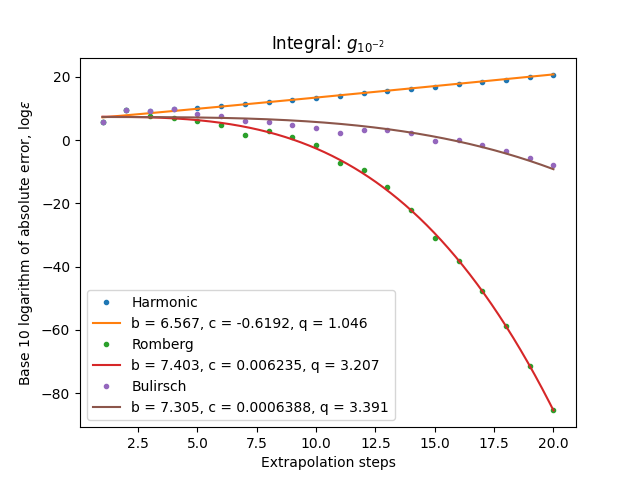
\includegraphics[scale=0.45]{romberg_plots/g_hundredth_hp_steps.png}
\end{minipage}
\end{figure}

\begin{figure}[H]
\centering
\begin{minipage}{0.45\textwidth}
\centering
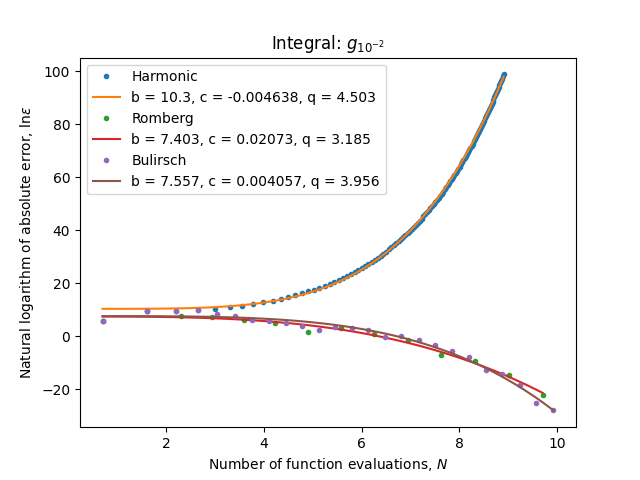
\includegraphics[scale=0.45]{romberg_plots/g_hundredth_hp_log_log_pow_fit_trend.png}
\end{minipage}
\begin{minipage}{0.45\textwidth}
\centering
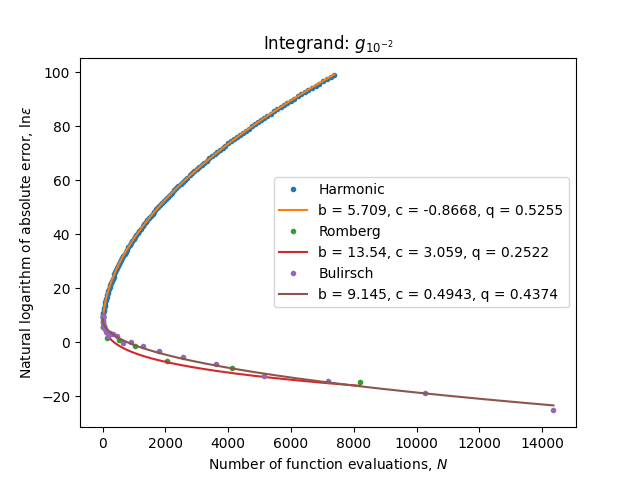
\includegraphics[scale=0.45]{romberg_plots/g_hundredth_hp_trend.png}
\end{minipage}
\end{figure}

\begin{table}[H]
    \centering
    \begin{tabular}{c|c||c|c|c}
Sequence & Plot & \(A\)-variance & \(c\)-variance & \(q\)-variance\\\hline
Harmonic & lin-ln evals-error & \(5.0593\) & \(0.042405\) & \(0.0071056\) \\
Romberg & lin-ln evals-error & \(nan\) & \(2.7999\) & \(1.0815\) \\
Bulirsch & lin-ln evals-error & \(nan\) & \(6.3194\) & \(1.1937\) \\
Harmonic & lin-ln steps-error & \(nan\) & \(111.94\) & \(0.012047\) \\
Romberg & lin-ln steps-error & \(4\) & \(3.1912\) & \(0.62642\) \\
Bulirsch & lin-ln steps-error & \(nan\) & \(3.4957\) & \(1.7296\) \\
Harmonic & ln-ln evals-error & . & . & . \\
Romberg & ln-ln evals-error & \(4\) & \(3.6997\) & \(0.68554\) \\
Bulirsch & ln-ln evals-error & \(nan\) & \(3.6555\) & \(1.8702\) \\
    \end{tabular}
    \label{tab:my_label}
\end{table}

Here the same comments apply as for \(a = 10^{-1}\), except that now the Romberg sequence performes better than the Bulirsch sequence and the model fitting is worse.

\subsection{Logarithm}

Now we will consider the following function 
\[
h_a: [0, 1] \rightarrow \R, \quad h_a(x) \coloneqq \ln(a + x),\, a > 0.
\]
This function is analytic on neighbourhood about the interval but we have a singularity at the horizontal ray from \(-a\) to \(-\infty\).

\begin{figure}[H]
\centering
\begin{minipage}{0.45\textwidth}
\centering
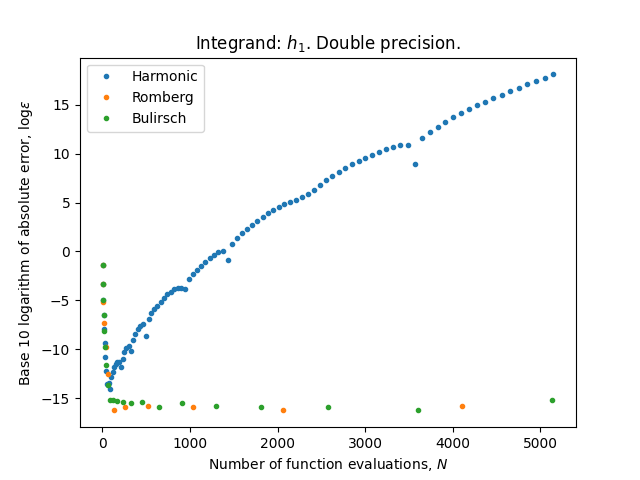
\includegraphics[scale=0.45]{romberg_plots/h_one.png}
\end{minipage}
\begin{minipage}{0.45\textwidth}
\centering
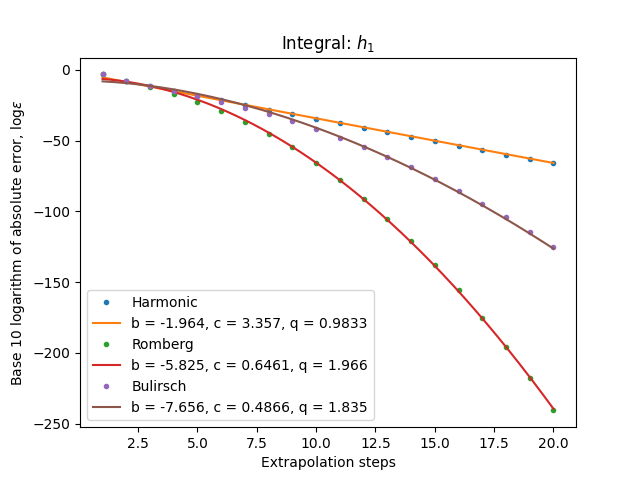
\includegraphics[scale=0.45]{romberg_plots/h_one_hp_steps.png}
\end{minipage}
\end{figure}

\begin{figure}[H]
\centering
\begin{minipage}{0.45\textwidth}
\centering
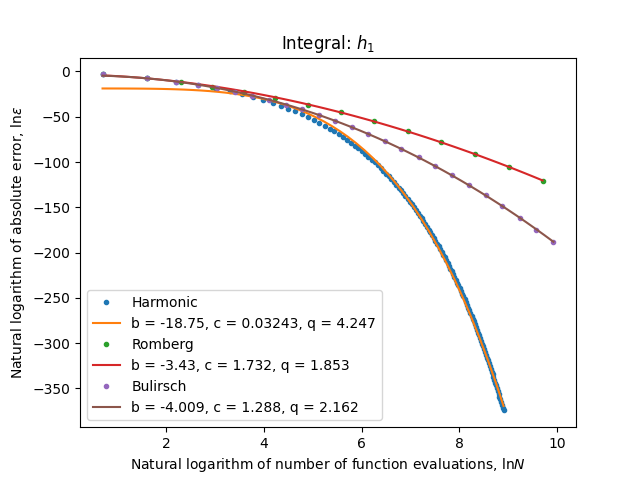
\includegraphics[scale=0.45]{romberg_plots/h_one_hp_log_log_pow_fit_trend.png}
\end{minipage}
\begin{minipage}{0.45\textwidth}
\centering
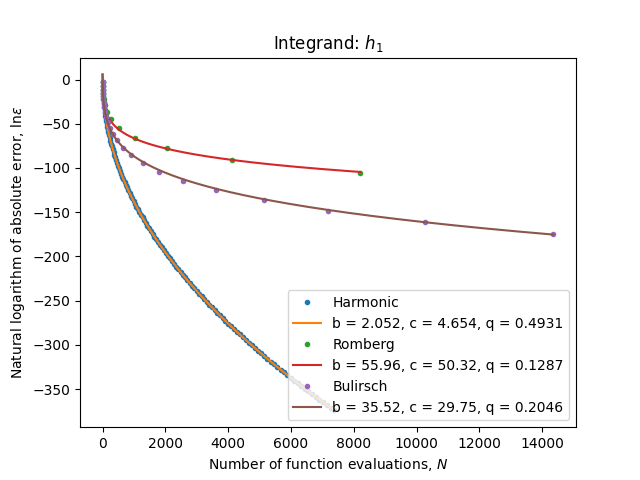
\includegraphics[scale=0.45]{romberg_plots/h_one_hp_trend.png}
\end{minipage}
\end{figure}

\begin{table}[H]
    \centering
    \begin{tabular}{c|c||c|c|c}
Sequence & Plot & \(A\)-variance & \(c\)-variance & \(q\)-variance\\\hline
Harmonic & lin-ln evals-error & \(1.6275\) & \(0.001334\) & \(8.4531e-05\) \\
Romberg & lin-ln evals-error & \(3.9961\) & \(0.034675\) & \(0.0095088\) \\
Bulirsch & lin-ln evals-error & \(13.729\) & \(0.23963\) & \(0.069978\) \\
Harmonic & lin-ln steps-error & \(3.3305\) & \(0.0028975\) & \(0.00016396\) \\
Romberg & lin-ln steps-error & \(0.94544\) & \(0.018617\) & \(0.00067321\) \\
Bulirsch & lin-ln steps-error & \(8.3957\) & \(0.32107\) & \(0.0068979\) \\
Harmonic & ln-ln evals-error & . & . & . \\
Romberg & ln-ln evals-error & \(1.1892\) & \(0.019677\) & \(0.0010134\) \\
Bulirsch & ln-ln evals-error & \(0.36829\) & \(0.0038072\) & \(0.00015789\) \\
    \end{tabular}
    \label{tab:my_label}
\end{table}

We see that the harmonic sequence performes best, then Bulirsch and then Romberg. In standard double precision arithmetic, we get down to machine level precision using Romberg or Bulirsch, but we are like \(2\) digits from there, using the harmonic sequence.\\

For the Romberg and Bulirsch sequence, we can not say that the error converges exponentially with the number of function evaluations. In the case of the harmonic sequence, the model seems to fit very well, since we have very little variance in the parameters.\\

For the harmonic sequence the error clearly seems to converge exponentally with the number of extrapolation steps, as we expect, since it seems to converge exponentially with the number of function evaluations. The exponent is approximately two the one from the former fitting as expected. The model, on the other hand, the fitting is rather unstable for the Romberg and Bulirsch sequence though, and hence also when considering the logarithm of the error against the logarithm of the number of function evaluations.

\begin{figure}[H]
\centering
\begin{minipage}{0.45\textwidth}
\centering
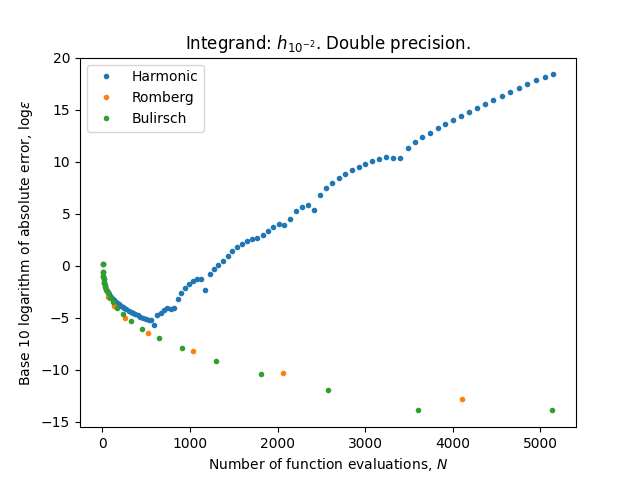
\includegraphics[scale=0.45]{romberg_plots/h_hundredth.png}
\end{minipage}
\begin{minipage}{0.45\textwidth}
\centering
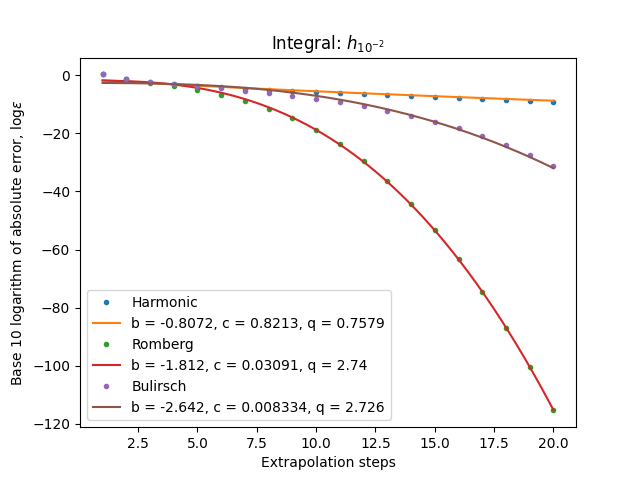
\includegraphics[scale=0.45]{romberg_plots/h_hundredth_hp_steps.png}
\end{minipage}
\end{figure}

\begin{figure}[H]
\centering
\begin{minipage}{0.45\textwidth}
\centering
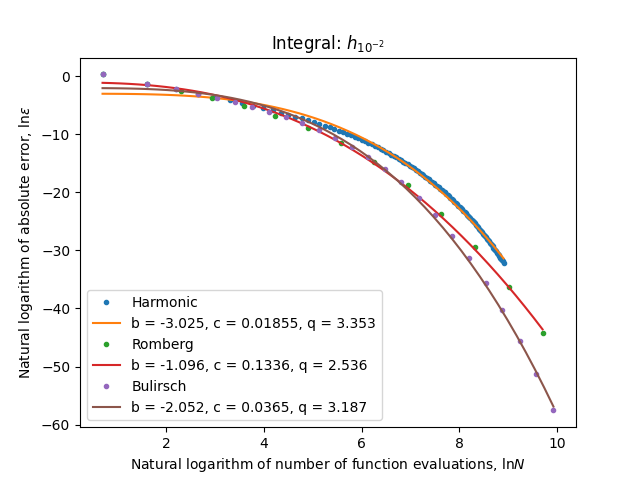
\includegraphics[scale=0.45]{romberg_plots/h_hundredth_hp_log_log_pow_fit_trend.png}
\end{minipage}
\begin{minipage}{0.45\textwidth}
\centering
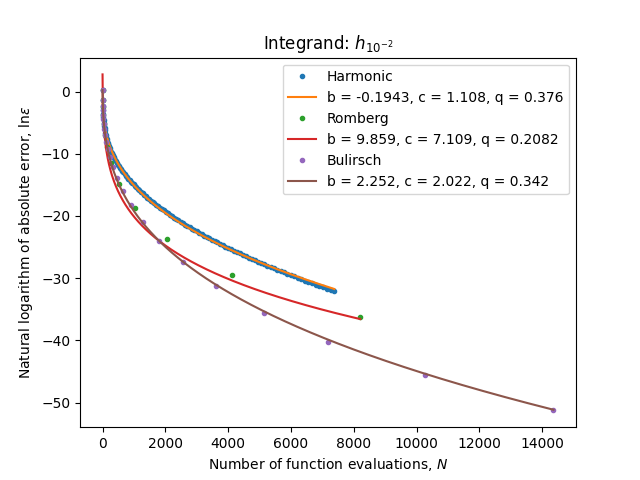
\includegraphics[scale=0.45]{romberg_plots/h_hundredth_hp_trend.png}
\end{minipage}
\end{figure}

\begin{table}[H]
    \centering
    \begin{tabular}{c|c||c|c|c}
Sequence & Plot & \(A\)-variance & \(c\)-variance & \(q\)-variance\\\hline
Harmonic & lin-ln evals-error & \(75.169\) & \(1.4423\) & \(0.030506\) \\
Romberg & lin-ln evals-error & \(1.9659\) & \(0.02769\) & \(0.002777\) \\
Bulirsch & lin-ln evals-error & \(10.207\) & \(0.15642\) & \(0.012213\) \\
Harmonic & lin-ln steps-error & \(26.823\) & \(1.0482\) & \(0.02436\) \\
Romberg & lin-ln steps-error & \(0.5511\) & \(0.3681\) & \(0.0061046\) \\
Bulirsch & lin-ln steps-error & \(2.8679\) & \(3.5395\) & \(0.047691\) \\
Harmonic & ln-ln evals-error & . & . & . \\
Romberg & ln-ln evals-error & \(0.62271\) & \(0.26181\) & \(0.0063053\) \\
Bulirsch & ln-ln evals-error & \(1.9572\) & \(1.649\) & \(0.028369\) \\
    \end{tabular}
    \label{tab:my_label}
\end{table}

We see that we can not attain high precision using the harmonic sequence and standard double precision. It is hard to tell which sequence performes best in the long run, though we can say that Bulirsch performes better than Romberg.\\

Here, none of our models seems to fit well. 

\begin{figure}[H]
\centering
\begin{minipage}{0.45\textwidth}
\centering
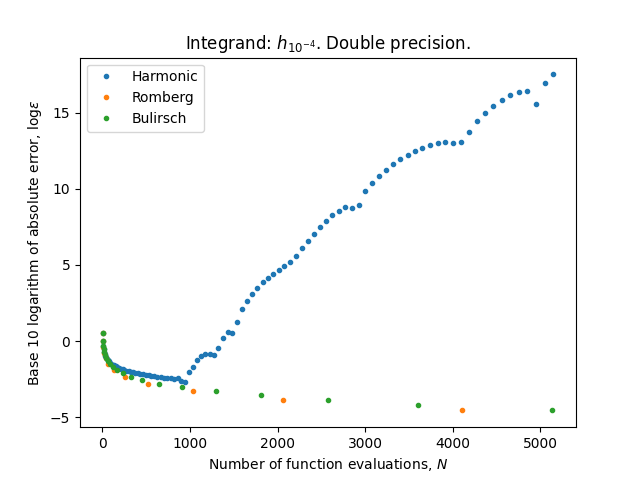
\includegraphics[scale=0.45]{romberg_plots/h_tenthousandth.png}
\end{minipage}
\begin{minipage}{0.45\textwidth}
\centering
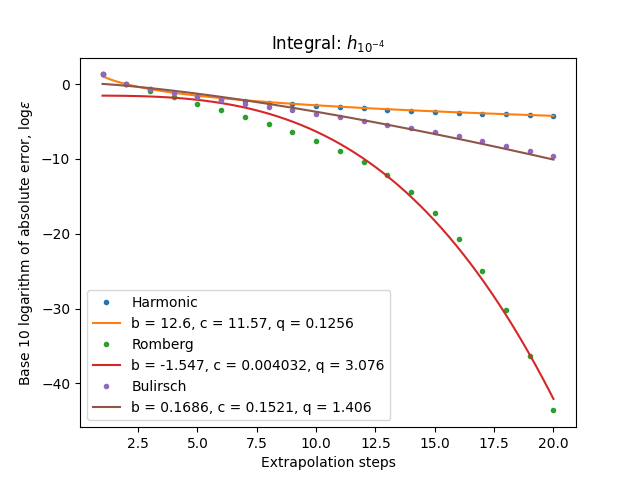
\includegraphics[scale=0.45]{romberg_plots/h_tenthousandth_hp_steps.png}
\end{minipage}
\end{figure}

\begin{figure}[H]
\centering
\begin{minipage}{0.45\textwidth}
\centering
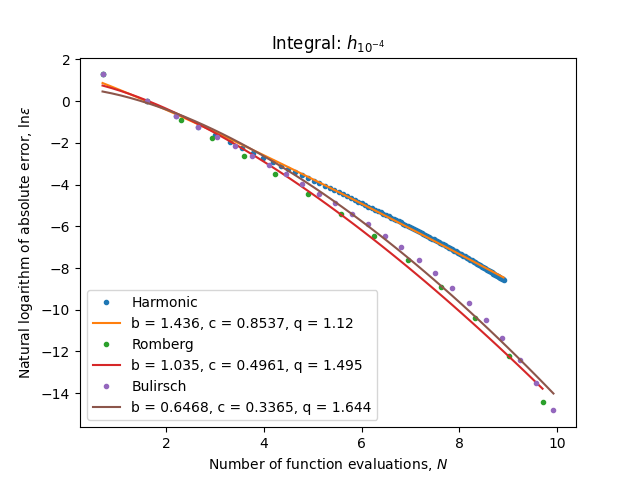
\includegraphics[scale=0.45]{romberg_plots/h_tenthousandth_hp_log_log_pow_fit_trend.png}
\end{minipage}
\begin{minipage}{0.45\textwidth}
\centering
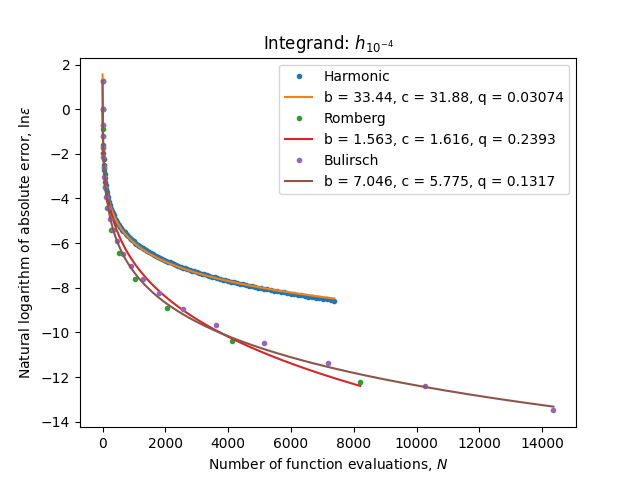
\includegraphics[scale=0.45]{romberg_plots/h_tenthousandth_hp_trend.png}
\end{minipage}
\end{figure}

\begin{table}[H]
    \centering
    \begin{tabular}{c|c||c|c|c}
Sequence & Plot & \(A\)-variance & \(c\)-variance & \(q\)-variance\\\hline
Harmonic & lin-ln evals-error & . & . & . \\
Romberg & lin-ln evals-error & \(3.9998\) & \(0.58702\) & \(0.20654\) \\
Bulirsch & lin-ln evals-error & \(3.8706\) & \(0.53846\) & \(0.31338\) \\
Harmonic & lin-ln steps-error & . & . & . \\
Romberg & lin-ln steps-error & \(0.79452\) & \(0.67424\) & \(0.054336\) \\
Bulirsch & lin-ln steps-error & \(1.3261\) & \(1.3702\) & \(0.15695\) \\
Harmonic & ln-ln evals-error & . & . & . \\
Romberg & ln-ln evals-error & \(1.0455\) & \(0.61797\) & \(0.065037\) \\
Bulirsch & ln-ln evals-error & \(1.0172\) & \(0.76715\) & \(0.15282\) \\
    \end{tabular}
    \label{tab:my_label}
\end{table}

Here again, we do not attain high precision when using the Harmonic sequence in double precision arithmetic. It is hard to say which sequence performes best. None of our models fits.

\subsection{Area of half circle}

Now we will try the following function:
\[
i: [-1, 1] \rightarrow \R, \quad i(x)\coloneqq \sqrt{1-x^2}.
\]
This function is analytic inside the interval of definition but not at the endpoints. Its derivative has singularities at the endpoints.

\begin{figure}[H]
\centering
\begin{minipage}{0.45\textwidth}
\centering
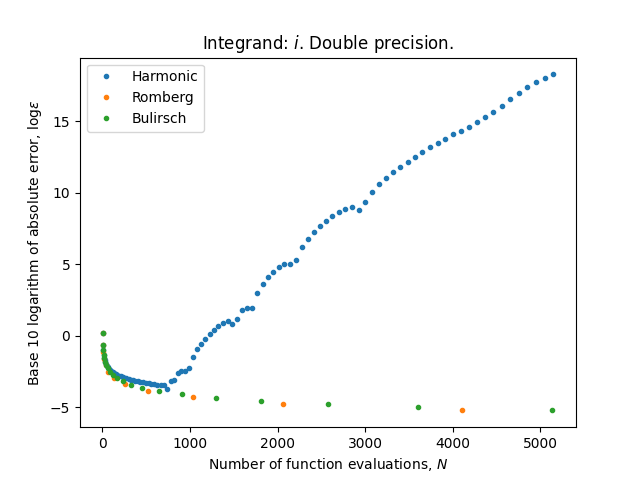
\includegraphics[scale=0.45]{romberg_plots/circle_area.png}
\end{minipage}
\begin{minipage}{0.45\textwidth}
\centering
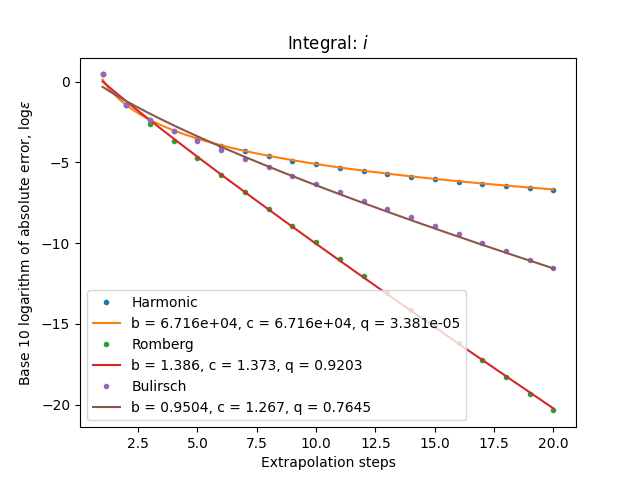
\includegraphics[scale=0.45]{romberg_plots/circle_area_hp_steps.png}
\end{minipage}
\end{figure}

\begin{figure}[H]
\centering
\begin{minipage}{0.45\textwidth}
\centering
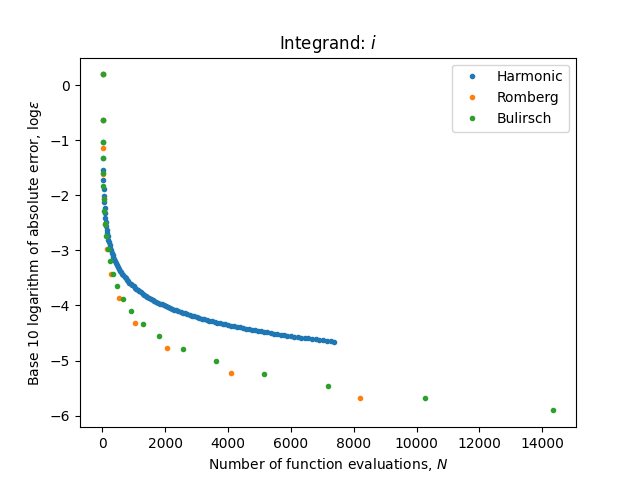
\includegraphics[scale=0.45]{romberg_plots/circle_area_hp.png}
\end{minipage}
\begin{minipage}{0.45\textwidth}
\centering
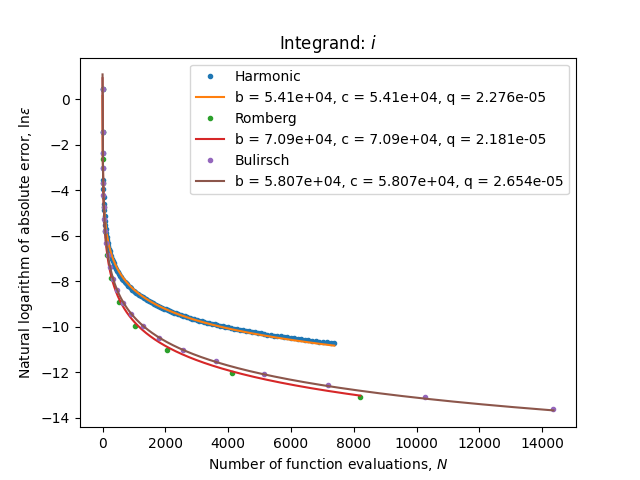
\includegraphics[scale=0.45]{romberg_plots/circle_area_hp_trend.png}
\end{minipage}
\end{figure}

\begin{table}[H]
    \centering
    \begin{tabular}{c|c||c|c|c}
Sequence & Plot & \(A\)-variance & \(c\)-variance & \(q\)-variance\\\hline
Harmonic & lin-ln evals-error & . & . & . \\
Romberg & lin-ln evals-error & \(nan\) & \(0.00074987\) & \(0.0010457\) \\
Bulirsch & lin-ln evals-error & . & . & . \\
Harmonic & lin-ln steps-error & . & . & . \\
Romberg & lin-ln steps-error & \(0.0017773\) & \(0.00025637\) & \(2.7817e-05\) \\
Bulirsch & lin-ln steps-error & \(0.16248\) & \(0.0448\) & \(0.003052\) \\
Harmonic & ln-ln evals-error & \(0.66509\) & \(0.035037\) & \(0.0039765\) \\
Romberg & ln-ln evals-error & \(0.11181\) & \(0.0085994\) & \(0.001262\) \\
Bulirsch & ln-ln evals-error & \(0.059168\) & \(0.0077593\) & \(0.001453\) \\
    \end{tabular}
    \label{tab:my_label}
\end{table}

We see that we do not get high precision using double precision arithmetic, independent of sequence. The Romberg and Bulirsch sequence seem to perform similarly well but the harmonic sequence seems to be slowest.\\

For the harmonic sequence, the error neither converges exponentally with the number of function evaluations nor the number of extrapolation steps. For the Bulirsch none of the models fits well, but for Romberg, model seems to fit moderately well when considering the logarithm of the error against the number of extrapolation steps or the logarithm of the number of function evaluations.

\subsection{Gaussian}

Finally we will consider the Gaussian function
\[
j: [0,1]\rightarrow \R, \quad k(x) \coloneqq \frac{2}{\sqrt{\pi}} e^{-x^2}.
\]
\begin{figure}[H]
\centering
\begin{minipage}{0.45\textwidth}
\centering
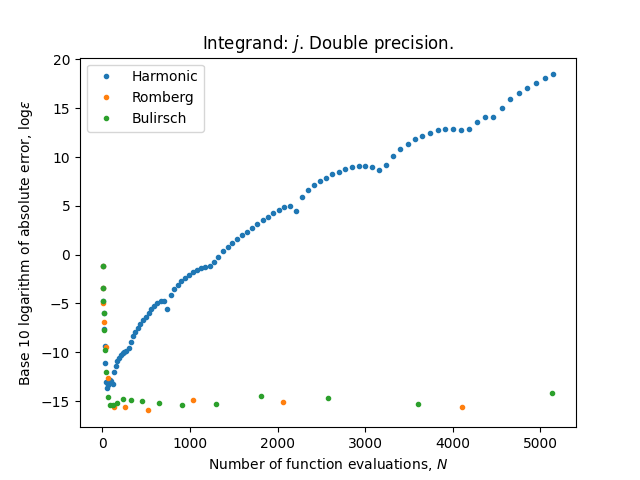
\includegraphics[scale=0.45]{romberg_plots/gaussian.png}
\end{minipage}
\begin{minipage}{0.45\textwidth}
\centering
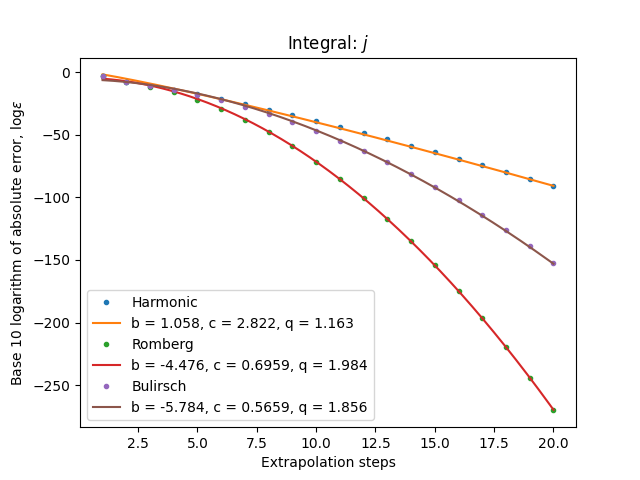
\includegraphics[scale=0.45]{romberg_plots/gaussian_hp_steps.png}
\end{minipage}
\end{figure}

\begin{figure}[H]
\centering
\begin{minipage}{0.45\textwidth}
\centering
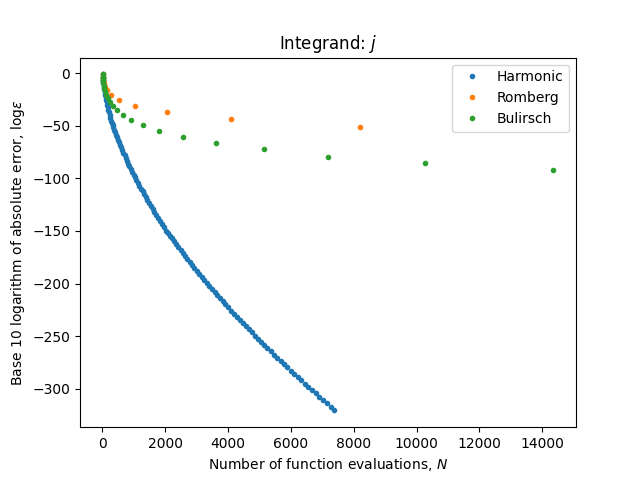
\includegraphics[scale=0.45]{romberg_plots/gaussian_hp.png}
\end{minipage}
\begin{minipage}{0.45\textwidth}
\centering
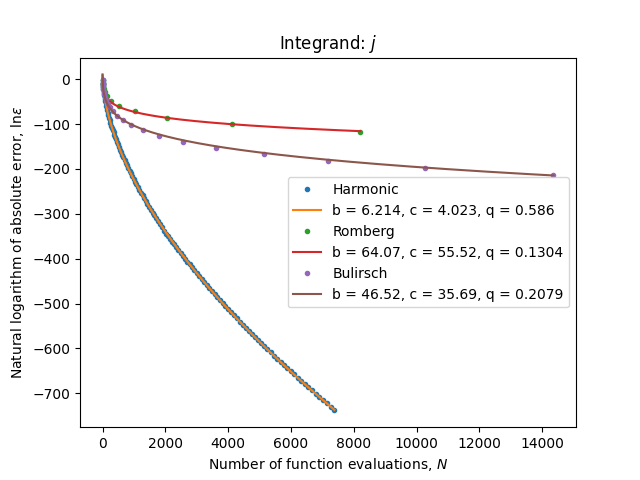
\includegraphics[scale=0.45]{romberg_plots/gaussian_hp_trend.png}
\end{minipage}
\end{figure}

\begin{table}[H]
    \centering
    \begin{tabular}{c|c||c|c|c}
Sequence & Plot & \(A\)-variance & \(c\)-variance & \(q\)-variance\\\hline
Harmonic & lin-ln evals-error & . & . & . \\
Romberg & lin-ln evals-error & \(3.9999\) & \(0.075546\) & \(0.02295\) \\
Bulirsch & lin-ln evals-error & \(nan\) & \(2.7536\) & \(0.17572\) \\
Harmonic & lin-ln steps-error & . & . & . \\
Romberg & lin-ln steps-error & \(0.023038\) & \(0.00025761\) & \(8.9728e-06\) \\
Bulirsch & lin-ln steps-error & \(15\) & \(1.1721\) & \(0.0087318\) \\
Harmonic & ln-ln evals-error & . & . & . \\
Romberg & ln-ln evals-error & \(0.16893\) & \(0.0015778\) & \(7.6206e-05\) \\
Bulirsch & ln-ln evals-error & \(15\) & \(1.4218\) & \(0.011922\) \\
    \end{tabular}
    \label{tab:my_label}
\end{table}

In double precision arithmetic we get down to machine level precision using Romberg or Bulirsch, but we get down to like \(2\) digits from there, using the harmonic sequence. The harmonic sequence performes best, then Bulirsch and then Romberg.\\

For the harmonic sequence, the error seems to converge exponentially with the number of extrapolation steps (and hence also with the number of extrapolation steps), but we though must note that there is quite a lot of variance in the \(b\) parameter and the \(c\) parameter. For the Romberg sequence, model fits moderately well when considering the logarithm of the error agains the number of extrapolation steps or the logarithm of the number of function evaluations. For the Bulirsch seqeunce, none of the models fits.

The values of the optimal parameters in the curve fitting of evaluations against the logarithm of the error are:

\begin{table}[H]
    \centering
    \begin{tabular}{c|c||c|c|c}
        Integrand & Sequence & \(b\) & \(c\) & \(q\) \\\hline\hline
$f$ & Harmonic & \(15.66\) & \(3.1537\) & \(0.63887\) \\
$f$ & Romberg & \(30.844\) & \(22.442\) & \(0.2014\) \\
$f$ & Bulirsch & \(46.309\) & \(29.549\) & \(0.22556\) \\
$g_{10^{-2}}$ & Harmonic & \(5.7088\) & \(-0.8668\) & \(0.52546\) \\
$g_{10^{-2}}$ & Romberg & \(9.3083\) & \(0.96199\) & \(0.35893\) \\
$g_{10^{-2}}$ & Bulirsch & \(9.1445\) & \(0.49433\) & \(0.43743\) \\
$g_{10^{-1}}$ & Harmonic & \(2.2352\) & \(-0.66129\) & \(0.51817\) \\
$g_{10^{-1}}$ & Romberg & \(9.3824\) & \(3.6029\) & \(0.29851\) \\
$g_{10^{-1}}$ & Bulirsch & \(10.844\) & \(2.8849\) & \(0.34731\) \\
$g_1$ & Harmonic & \(1.6178\) & \(1.823\) & \(0.49467\) \\
$g_1$ & Romberg & \(23.192\) & \(18.171\) & \(0.19817\) \\
$g_1$ & Bulirsch & \(24.613\) & \(15.795\) & \(0.24492\) \\
$h_{10^{-4}}$ & Harmonic & \(33.436\) & \(31.879\) & \(0.030738\) \\
$h_{10^{-4}}$ & Romberg & \(9.6285\) & \(8.0889\) & \(0.1106\) \\
$h_{10^{-4}}$ & Bulirsch & \(7.0462\) & \(5.7755\) & \(0.13169\) \\
$h_{10^{-2}}$ & Harmonic & \(-0.19426\) & \(1.1078\) & \(0.37602\) \\
$h_{10^{-2}}$ & Romberg & \(4.3792\) & \(3.631\) & \(0.26761\) \\
$h_{10^{-2}}$ & Bulirsch & \(2.2519\) & \(2.0217\) & \(0.34203\) \\
$h_1$ & Harmonic & \(2.052\) & \(4.6543\) & \(0.4931\) \\
$h_1$ & Romberg & \(33.542\) & \(31.468\) & \(0.16462\) \\
$h_1$ & Bulirsch & \(35.525\) & \(29.752\) & \(0.20461\) \\
$i$ & Harmonic & \(54099\) & \(54099\) & \(2.2756\cdot 10^{-5}\) \\
$i$ & Romberg & \(55368\) & \(55367\) & \(2.8621\cdot 10^{-5}\) \\
$i$ & Bulirsch & \(58074\) & \(58073\) & \(2.6538\cdot 10^{-5}\) \\
$j$ & Harmonic & \(6.2138\) & \(4.0228\) & \(0.58595\) \\
$j$ & Romberg & \(33.68\) & \(30.265\) & \(0.17797\) \\
$j$ & Bulirsch & \(46.521\) & \(35.69\) & \(0.20788\) \\
    \end{tabular}
    \caption{Optimal parameters by test case}
    \label{tab:my_label}
\end{table}

The values of the optimal parameters in the curve fitting of extrapolation steps against the logarithm of the error are:

\begin{table}[H]
    \centering
    \begin{tabular}{c|c||c|c|c}
        Integrand & Sequence & \(b\) & \(c\) & \(q\) \\\hline\hline
$f$ & Harmonic & \(10.466\) & \(2.1696\) & \(1.2654\) \\
$f$ & Romberg & \(1.5206\) & \(0.51255\) & \(2.089\) \\
$f$ & Bulirsch & \(0.77673\) & \(0.41734\) & \(1.9549\) \\
$g_{10^{-2}}$ & Harmonic & \(6.5675\) & \(-0.61916\) & \(1.0458\) \\
$g_{10^{-2}}$ & Romberg & \(7.3378\) & \(0.0066103\) & \(3.1744\) \\
$g_{10^{-2}}$ & Bulirsch & \(7.3047\) & \(0.00063882\) & \(3.3913\) \\
$g_{10^{-1}}$ & Harmonic & \(2.8699\) & \(-0.47343\) & \(1.0317\) \\
$g_{10^{-1}}$ & Romberg & \(3.1888\) & \(0.039167\) & \(2.7667\) \\
$g_{10^{-1}}$ & Bulirsch & \(3.9142\) & \(0.012441\) & \(2.7293\) \\
$g_1$ & Harmonic & \(0.034332\) & \(1.3144\) & \(0.98632\) \\
$g_1$ & Romberg & \(-0.4289\) & \(0.41763\) & \(2.0726\) \\
$g_1$ & Bulirsch & \(-1.3077\) & \(0.18952\) & \(2.0725\) \\
$h_{10^{-4}}$ & Harmonic & \(12.604\) & \(11.571\) & \(0.12559\) \\
$h_{10^{-4}}$ & Romberg & \(0.85129\) & \(0.27953\) & \(1.4991\) \\
$h_{10^{-4}}$ & Bulirsch & \(0.16861\) & \(0.15206\) & \(1.4061\) \\
$h_{10^{-2}}$ & Harmonic & \(-0.80722\) & \(0.82135\) & \(0.75792\) \\
$h_{10^{-2}}$ & Romberg & \(-1.309\) & \(0.051824\) & \(2.5402\) \\
$h_{10^{-2}}$ & Bulirsch & \(-2.6424\) & \(0.0083341\) & \(2.7259\) \\
$h_1$ & Harmonic & \(-1.9642\) & \(3.3575\) & \(0.98328\) \\
$h_1$ & Romberg & \(-4.397\) & \(0.86863\) & \(1.8535\) \\
$h_1$ & Bulirsch & \(-7.6558\) & \(0.48664\) & \(1.8348\) \\
$i$ & Harmonic & \(67160\) & \(67160\) & \(3.3808\cdot 10^{-5}\) \\
$i$ & Romberg & \(1.8004\) & \(1.6494\) & \(0.85593\) \\
$i$ & Bulirsch & \(0.95043\) & \(1.2669\) & \(0.7645\) \\
$j$ & Harmonic & \(1.0579\) & \(2.8215\) & \(1.1626\) \\
$j$ & Romberg & \(-3.906\) & \(0.77717\) & \(1.9416\) \\
$j$ & Bulirsch & \(-5.7837\) & \(0.56594\) & \(1.8564\)
    \end{tabular}
    \caption{Optimal parameters by test case}
    \label{tab:my_label}
\end{table}